\documentclass[11pt]{article}
\usepackage[margin=2.5cm]{geometry}
\usepackage{amsmath,amssymb}
\usepackage{graphicx}
\usepackage{xcolor}
\usepackage{booktabs}
\usepackage{pdfpages}
\usepackage{algorithm}
\usepackage{algpseudocode}
\usepackage{authblk}
\usepackage[colorlinks=true,linkcolor=blue,citecolor=blue,urlcolor=blue]{hyperref}

\newcommand{\pstick}{p_{\mathrm{stick}}}
\newcommand{\dt}{\Delta t}
\graphicspath{{results/}{./}}
\setlength{\emergencystretch}{2em}

\newcommand{\fillin}[1]{\textcolor{red}{[#1]}}




\title{Report for Project 3}
\author[1]{Javad Yousefian}
\author[1]{Alexandra VonHaven}
\author[1]{Kevin Geumhan}
\affil[1]{Department of Physics, Syracuse University, Syracuse, New York 13244, USA}
\date{}
\begin{document}
\maketitle
\begin{abstract}
Markov chain Monte Carlo (MCMC) methods were used to sample the imaginary-time
path integral of a quantum harmonic oscillator. A periodic lattice with
$N = 64$ time slices was implemented, resulting in a 64-dimensional Gaussian
distribution with available exact results. A checkerboard Metropolis sampler
was developed and its performance evaluated against the \texttt{emcee} sampler.
A validation plan was established and refined throughout code development.
Twelve validation tests were performed, all of which were successful. Both
samplers produced results consistent with the exact lattice calculations and
with each other within $1.3\sigma$. For four chains, the largest
rank-normalized $\hat R$ was $1.0037$. An injection test accurately recovered
the input mass and frequency within $2.1\sigma$ across five lattices and
rejected an incorrect frequency at $9.7\sigma$. Additionally, six intentional
bugs were introduced, each detected by at least one validation test.
\end{abstract}

\section{Original Validation Plan}
\subsection{Introduction}
In this project, we plan to sample the path integral of the quantum harmonic oscillator in imaginary time using Markov chain Monte Carlo methods. We will write our own Metropolis sampler and also use \texttt{emcee}~\cite{emcee} so we can directly compare the two methods. This document describes our code validation plan and was written before any code, so it does not include results.

Our main goal is to check if our Metropolis code samples the correct distribution. The harmonic oscillator is a good choice for validation because its lattice distribution is Gaussian, which lets us compare with exact analytical results. 

\subsection{The Model}
The Euclidean action of the oscillator is
\begin{equation}
  S_E = \int_0^{T_\tau} d\tau \left[ \frac{m}{2}\dot x^2 + \frac{m\omega^2}{2}x^2 \right].
\end{equation}
We divide the time into $N$ steps of size $\epsilon$ and use this discretization and rescaling:
\begin{equation}
  a = \omega\epsilon, \qquad \kappa = \frac{a^2}{4}, \qquad g = \frac{1-\kappa}{1+\kappa}, \qquad x_j = \sqrt{\frac{\hbar\epsilon}{m(1+\kappa)}}\, u_j .
\end{equation}
The endpoints are fixed, $u_0 = u_N = 0$, so the free variables are $u_1, \dots, u_{N-1}$. This is $D = N-1$ dimensions ($D = 63$ for our main lattice). The action becomes
\begin{equation}
  \mathcal S(u) = \sum_{j=1}^{N-1} u_j^2 - g \sum_{j=0}^{N-1} u_j u_{j+1},
  \label{eq:action}
\end{equation}
and we sample $\pi(u) \propto e^{-\mathcal S(u)}$. We keep the endpoints fixed and do not use periodic boundaries, because that would change the distribution.

\paragraph{Exact Solution.} The action can be written as $\mathcal S = \frac12 u^T Q u$, where $Q$ has 2 on the diagonal and $-g$ next to the diagonal. Since $|g| < 1$, $Q$ is positive definite, so $\pi$ is a Gaussian with mean zero and covariance $Q^{-1}$:
\begin{equation}
  \langle u_j \rangle = 0, \qquad \langle u_j u_k \rangle = (Q^{-1})_{jk}, \qquad \langle u_j^4 \rangle = 3 \left[(Q^{-1})_{jj}\right]^2 .
  \label{eq:exact}
\end{equation}
We can get $Q^{-1}$ from NumPy, but there is also a closed formula for it. With $\mu = 2\,\mathrm{artanh}(a/2)$,
\begin{equation}
  (Q^{-1})_{jk} = \frac{\sinh(\mu \min(j,k))\, \sinh(\mu(N-\max(j,k)))}{g \sinh\mu \, \sinh(\mu N)} .
  \label{eq:Qinv}
\end{equation}
Far from the ends this is about $\frac{1+\kappa}{2a}\rho^{|j-k|}$ with $\rho = (2-a)/(2+a)$. For $a = 0.25$ this gives $\langle u_j^2\rangle \approx 2.03$, $\langle u_j u_{j+1}\rangle \approx 1.58$ and $\langle u_j u_{j+2}\rangle \approx 1.23$. Near the ends the variance is smaller: for $a = 0.25$ it is 0.802 at $j = 1$, 1.288 at $j = 2$ and 1.759 at $j = 4$.



\paragraph{Symmetries.} The distribution does not change if we flip the sign of the path ($u \to -u$) or if we reverse it in time ($u_j \to u_{N-j}$). So $\langle u_j\rangle = 0$ and $\langle u_j u_k\rangle = \langle u_{N-j}u_{N-k}\rangle$. There are no degeneracies, because $Q$ is positive definite and there is only one peak, at $u = 0$.

\paragraph{Energy Gap.} In the middle of the lattice the correlation falls like $\rho^k$, so the decay rate per unit time is
\begin{equation}
  \frac{\omega_{\text{lat}}}{\omega} = \frac{2}{a}\,\mathrm{artanh}\!\left(\frac a2\right).
  \label{eq:wlat}
\end{equation}
For small $a$ this goes to 1, which is the continuum gap $E_1 - E_0 = \hbar\omega$. At $a = 1$ it is 1.099.

\subsection{What the Code Will Do}
\begin{enumerate}
  \item Make a path with $u_0 = u_N = 0$ and compute its action, Eq.~\eqref{eq:action}.
  \item Sample the path with our Metropolis code, and separately with \texttt{emcee}.
  \item Measure $\langle u_j\rangle$, $\langle u_j^2\rangle$, $\langle u_j^4\rangle$ and the correlation $\langle u_{j_0} u_{j_0+k}\rangle$, where $j_0 = N/2$ is the middle site.
  \item Fit the decay of the correlation to get the energy gap.
  \item Compute error bars and convergence checks.
  \item Save the settings, the seed, the results and the plots, so every run can be repeated.
\end{enumerate}

\subsection{Samplers}
\paragraph{Our Metropolis sampler.} In one sweep we go through all sites $j = 1, \dots, N-1$. For each site we propose $u_j' = u_j + \delta$, with $\delta$ uniform in $[-\Delta, \Delta]$. The change of the action only depends on the two neighbours:
\begin{equation}
  \Delta\mathcal S = \delta\,[\delta + 2u_j - g(u_{j-1}+u_{j+1})].
  \label{eq:dS}
\end{equation}
We accept with probability $\min(1, e^{-\Delta \mathcal S})$. If we reject, we keep the old value and still count it as the next sample. To make it faster, we update all odd sites at the same time and then all even sites. This is allowed because odd sites are not neighbours of each other.

The expected acceptance rate can also be calculated exactly. Given its neighbours, $u_j$ is Gaussian with variance $1/2$ (for any $a$ and $N$), and averaging over this gives
\begin{equation}
  A(\Delta) = \mathrm{erfc}\!\left(\frac\Delta 2\right) + \frac{2}{\sqrt\pi\,\Delta}\left(1 - e^{-\Delta^2/4}\right).
  \label{eq:acc}
\end{equation}
For example $A(1) = 0.729$, $A(2) = 0.514$ and $A(3) = 0.370$. It does not depend on $a$, so the acceptance should be the same for every lattice spacing.

We will try $\Delta = 0.5$, 1, 1.5, 2, 2.5, 3, and 4 in short pilot runs. After that, we will choose the value that gives the most effective samples with an acceptance rate between about 35\% and 65\%. We expect this value to be around 2.5.

\paragraph{emcee.} For the second sampler, we use \texttt{emcee.EnsembleSampler} with the same log probability $-\mathcal S(u)$ and at least $2D$ walkers. Because emcee works differently from our sampler, we expect the averages to match but not the individual chains. emcee is slow in high dimensions, so we will mainly use it for $N = 64$. If it is too slow, we will switch to $N = 16$ and note this change in the report. We will run emcee four times independently so we can compute $\hat R$.

\paragraph{Settings.} Our main lattice is $N = 64$ and $a = 0.25$, so $T = Na = 16$. For the energy gap test, we also use $N = 16$ with $a = 1$, and $N = 32$ with $a = 0.5$. We start four chains, each with 8,000 sweeps of burn-in and 40,000 sweeps for sampling. If the convergence checks fail, we will run longer. Two chains start at $u = 0$, and the other two start from a random path that is much wider than the real distribution.

\subsection{Error Bars and Passing Conditions}
Our samples are correlated, so we cannot use the normal $\sigma/\sqrt{M}$ error. We compute the integrated autocorrelation time
\begin{equation}
  \tau_{\text{int}} = \frac12 + \sum_{\ell=1}^{\ell_{\max}} \rho(\ell),
\end{equation}
where $\rho(\ell)$ is the autocorrelation at lag $\ell$ and $\ell_{\max}$ is chosen with Sokal's window~\cite{sokal}. The effective sample size is then $M/(2\tau_{\text{int}})$ for $M$ samples. emcee uses $1 + 2\sum\rho$, which is $2\tau_{\text{int}}$, so we divide emcee's number by 2. For the error bars we use batch means, with batches at least $20\tau_{\text{int}}$ long.

For the statistical tests we compare with the exact value using
\begin{equation}
  z = \frac{|\text{measured} - \text{exact}|}{\text{error bar}},
\end{equation}
and a test passes if $z \le 3.5$. We do many comparisons, so one of them could fail just by chance. If that happens, we run the test again with a different seed before we decide that there is a bug, and we report both runs. We will not change these limits after we see the results.

\subsection{Tests}
For every test we write what we check, when it passes, and what it would mean if it fails.

\subsubsection*{Test 1: Action and the Update}
We compare $\Delta\mathcal S$ from Eq.~\eqref{eq:dS} with the difference of the full action for 1000 random paths. They should agree to $10^{-10}$. We also check that $\frac12 u^T Q u$ gives the same action, that the acceptance probability is always between 0 and 1, and that the fast odd/even sweep gives exactly the same result as a simple loop over the sites when we give both the same random numbers. If this fails, there is probably a sign or index mistake, or a problem at the endpoints.

\subsubsection*{Test 2: Exact Covariance}
We check that our $Q$ is symmetric and positive definite, that its eigenvalues are $2 - 2g\cos(r\pi/N)$ for $r = 1, \dots, N-1$, and that the closed formula Eq.~\eqref{eq:Qinv} agrees with NumPy's inverse to $10^{-10}$. For $a = 0.25$ the numbers should match the values in Section 2. All the other tests compare with this, so if it fails we fix it first.

\subsubsection*{Test 3: Error Bars}
Before we trust our error bars, we test the autocorrelation and batch-means code on AR(1) data, $x_t = \phi x_{t-1} + \sqrt{1-\phi^2}\,\epsilon_t$, where the exact answer is $\tau_{\text{int}} = (1+\phi)/(2(1-\phi))$. We use $\phi = 0.5$, 0.9 and 0.99. The estimate of $\tau_{\text{int}}$ should be within 10\%, the batch-means error within 20\%, and emcee's value should be about $2\tau_{\text{int}}$. We also check that $\hat R$ is below 1.01 for four normal chains and above 1.01 if we shift one of them. If this fails, none of our error bars can be trusted.

\subsubsection*{Test 4: Very Small Lattices}
For $N = 2$ there is only one variable, and it should be Gaussian with variance $1/2$. For $N = 3$ there are two variables, and $u_1+u_2$ and $u_1-u_2$ should be independent Gaussians with variances $2/(2-g)$ and $2/(2+g)$. We run 200,000 sweeps and do a Kolmogorov--Smirnov test against these Gaussians, which passes if $p > 0.001$. The variance, the fourth moment and the acceptance rate should also pass $z \le 3.5$. This test can find mistakes that Test 1 cannot, for example if we forget to save the old value when a step is rejected.

\subsubsection*{Test 5: Known Answer at $N = 64$}
This is the main test. With $N = 64$ and $a = 0.25$ we measure $\langle u_{j_0}\rangle$, $\langle u_{j_0}u_{j_0+k}\rangle$ for $k = 0, 1, 2, 4, 8$, $\langle u_{j_0}^4\rangle$, and the variance at the sites near the ends ($j = 1, 2, 4$ and $N-4$, $N-2$, $N-1$). All of them should pass $z \le 3.5$ against Eq.~\eqref{eq:exact}. If something fails, the sampler is biased, there is a bug near the ends, or our error bars are wrong.

\subsubsection*{Test 6: Symmetries and Starting Points}
Because of the symmetries, $\langle u_j\rangle$ should be zero at $j = N/4$, $N/2$ and $3N/4$, and $\langle u_{j_0}u_{j_0+4}\rangle$ should be equal to $\langle u_{j_0}u_{j_0-4}\rangle$. We also compare the chains that started at $u = 0$ with the ones that started from a wide random path, and they should agree within 3 error bars. If not, the burn-in is too short, the chains do not mix well, or a bug breaks one of the symmetries.

\subsubsection*{Test 7: Convergence}
We look at trace plots of $u_{j_0}$, $u_{j_0}^2$ and the path average $\bar u$. The path average changes the slowest, so it is the most important one. For all the numbers we report, we need $\hat R < 1.01$ (the rank-normalized split $\hat R$ from~\cite{vehtari}) and an effective sample size above 400 in total. If this fails, we run longer or change $\Delta$.

\subsubsection*{Test 8: Acceptance Rate}
For each $\Delta$ in the pilot runs, the measured acceptance should agree with $A(\Delta)$ from Eq.~\eqref{eq:acc} ($z \le 3.5$), both for $a = 0.25$ and for $a = 1$. Since $A$ does not depend on $a$, both should give the same numbers. If it fails, there is a mistake in the $\delta^2$ part of $\Delta\mathcal S$, in the proposal width, or in the accept/reject step.

\subsubsection*{Test 9: Our Sampler Against emcee}
We compare $\langle u_{j_0}\rangle$, $\langle u_{j_0}^2\rangle$ and the correlation at $k = 1, 4, 8$ from our sampler and from emcee at $N = 64$. The difference divided by the combined error bar should be at most 3. Both samplers should also agree with the exact answer, because two samplers can agree with each other and still both be wrong. If one of them does not converge, we do not use it to judge the other one.

\subsubsection*{Test 10: Getting Back the Energy gap}
This is our injection test: we put $\omega$ into the code (through $a$), and we check that we get it back from the samples. For $a = 1$, 0.5 and 0.25 (all with $T = 16$) we fit $\langle u_{j_0}u_{j_0+k}\rangle \propto e^{-\hat\mu k}$ for times $ka$ between 0.5 and 3, using the middle part of the lattice. Then $\hat\mu/a$ should agree with Eq.~\eqref{eq:wlat} within 3.5 error bars, and the fit should be good ($p > 0.001$). At $a = 1$ the lattice value 1.099 is about 10\% above the continuum value, so we hope to see this difference. If the test fails, the fit is wrong or the sampler is biased at long distances.

\subsubsection*{Test 11: Multi-Walker Test}
We run the mcmc code for multiple walkers. After the burn-in period, we record the fraction of remaining sweeps that each walker stayed within a certain interval. If the code is valid, each walker should stay within a given region for roughly the same amount of time. 


\subsection{Test Execution}
When we write the code, we will turn these tests into \texttt{pytest} files where possible, so they can run automatically. Tests 1--4 and 8 are fast and will run on every pull request. Tests 5--7 need longer runs, and Tests 9 and 10 will be in a separate script. We have to look at the trace plots in Test 7 ourselves.

\subsection{Workflow}
We will add this plan to our Git repository before we start coding, so the Git history shows that the plan came before the code. After that, all changes (including code, tests, and this plan) will go through pull requests, and the other person will review them in writing before merging.

If a test fails or is not useful, we will update the plan in a new commit and keep the old version in the history. The commit message and the report will explain what changed and why. 

\subsection{Validation Plan Revisions}

\begin{table}[htbp]
\centering
\footnotesize
\setlength{\tabcolsep}{3pt}
\begin{tabular}{p{1.1cm}p{1.7cm}p{7.8cm}p{3.8cm}}
\toprule
Version & Commit & What changed & Why\\
\midrule
v1 \newline Nov 10 & 9063227 &
The original plan: fixed endpoints, Metropolis and \texttt{emcee}, Tests 1--10. &
This version was prepared before implementation.\\[2pt]
v1.1 \newline Nov 14 & 4ef6b7d &
Test 11 (multi-walker test) added. The new test runs a specified number of
walkers and determines how long each walker stays in the intervals
$[-\infty, -1]$, $[-\frac12,\frac12]$, $[\frac12, 1]$, and $[1, \infty]$.
The code assumes a burn-in period of 1000 iterations and calculates the
fraction of the total post-burn-in iterations each walker was within each of
these given intervals. The main plot shows the fraction of time spent in each
region for the walkers over the expected values based on the lattice produced
by the \texttt{exact\_correlator} function in \texttt{verify\_sho.py} as well
as the analytical continuum value for the quantum harmonic oscillator. We
included an additional plot showing how well the walkers agree with one
another more directly by plotting the standard deviation. The plot highlights
where the standard deviation is for the whole set. &
\\[2pt]
v1.2 \newline Nov 14 & d8dcc13 &
Tests 6 and 8 rewritten for the periodic lattice; pass limits for Test 11.
On the periodic lattice, there are no longer end sites. There is an additional
symmetry present when shifting the path in time $x_t\to x_{t+s}$. Time
reversal is now defined as $x_t \to x_{N-t}$. The pass threshold for each check
is also specified. A second multi-walker test file was created. It runs 8000
burn-in sweeps and keeps the subsequent 40,000. The script tests the path
average instead of averaging over all sites at every sweep. It also gives a
clearer pass/fall verdict than the previous test. &
The code samples a periodic lattice instead of using fixed endpoints and
measures the step size in alternative units.\\[2pt]
v1.3 \newline Nov 15 & 2bdc52d, 0615203 \newline (again: dde214f, 5a48677) &
Sections 3, 4, 5 and 7 and Test 10 rewritten for the periodic code; Test 10
recovers $m$ and $\omega$, with a negative control; commands instead of
\texttt{pytest}. The initial version of this test employed the fixed-endpoint
lattice and its energy-gap formula. The current code samples the periodic
lattice with the action
$S=\sum_t\big[\tfrac{m}{2a}(x_{t+1}-x_t)^2+\tfrac{a m\omega^2}{2}x_t^2\big]$. &
The same mismatch persisted; recovering both input parameters tests a broader
portion of the code. Our tests are statistical runs with retained
outputs.\\[2pt]
v1.4 \newline Nov 16 & b499b66 &
Section 2 written for the periodic lattice; Tests 1--5, 7 and 9 and the
\texttt{emcee} paragraph changed to match the code; Test 4 uses only $N = 2$;
the whole plan reworded in a more formal style. The wording of the whole plan
was also made more formal; the content of the other sections did not change. &
To fully align the plan with the code; the checkerboard update requires an even
$N$.\\[2pt]
v1.5 \newline Nov 16 & 58ad912, 321bd64 &
Test 12 added: six bugs put into a copy of the code on purpose; Section 7 lists
the command for every test. &
Until then, only the negative control had demonstrated that a test could
fail.\\
\bottomrule
\end{tabular}
\caption{Versions of the validation plan, with the dates of their commits
(\texttt{git log -{}- Validation*}). The plan text gives the dates on which
v1.3 and v1.4 were written, one day earlier.}
\label{tab:versions}
\end{table}

\paragraph{v1.1.} Alex introduced Test 11 to evaluate multiple walkers.
After burn-in, we measured the fraction of time each walker spent within a
specified interval. Accurate sampling requires that all walkers yield
comparable fractions. The initial script executed six walkers from distinct
starting positions, compared their $\langle x^2\rangle$ values and time
fractions in various regions to the exact Gaussian distribution, and computed
$\hat R$. In v1.2, we incorporated numerical pass limits.

\paragraph{v1.2.} By November 14, the code sampled a periodic lattice, whereas
the initial plan used fixed endpoints and a rescaled action. We updated Tests 6
and 8 to match the actual lattice. For a periodic lattice, time translation is
also a symmetry. We also corrected the step-size conversion:
$\delta = \Delta/\sqrt{A}$. For Test 11, each walker's fraction of time inside
$|q| < \sigma_q$ must agree with $\mathrm{erf}(1/\sqrt2) = 0.6827$ within
$3.5\sigma$, and the comparison among walkers must yield $p > 10^{-3}$.

\paragraph{v1.3.} We revised the sections detailing the model, sampler
settings, error analysis, and test execution procedures. Test 10 was
also modified: instead of estimating only the energy gap, it now employs five
lattices with known mass and frequency, fitting both parameters from the
correlator. Both parameters must be recovered within $3.5\sigma$, and the fit
must yield $p > 10^{-3}$. We introduced a negative control with input
$\omega = 1.1$, compared to $\omega = 1$; this control is required to fail. We
used package commands instead of separate \texttt{pytest} files, as our tests
involve statistical simulations, figures, and saved results. The v1.3 commits
were inadvertently pushed twice, resulting in two sets of commits with
identical content.

\paragraph{v1.4.} We also updated the plan to describe the periodic lattice and
its exact covariance and energy formulas. Tests 1--5, 7, and 9, and the
description of \texttt{emcee} were updated accordingly. Since checkerboard
updates require even $N$, we removed the $N = 3$ case from Test 4. The
remaining $N = 2$, $a = 1$ test uses the independent Gaussian variables
$x_0 + x_1$ and $x_0 - x_1$, whose variances are 2 and 0.4. We also edited the
wording of the plan. These changes were committed together.

\paragraph{v1.5.} We aimed to ensure that the tests could detect incorrect
code, not merely confirm correct code. We added Test 12, in which six distinct
bugs were introduced individually into a temporary copy of the package. For
each bug, at least one validation test was required to fail. The commands for
running the tests were also included in Section 7 of the plan.


\section{Model and Sampling Method}\label{sec:model}

\subsection{The Physical Problem}

We consider a one-dimensional quantum harmonic oscillator with mass $m$ and
angular frequency $\omega$. We use units where $\hbar = 1$. In imaginary time,
each path $x(\tau)$ has weight $e^{-S_E[x]}$, where the Euclidean action is
\begin{equation}
  S_E[x] = \int_0^{T} d\tau \left[ \frac{m}{2}\dot{x}^2
           + \frac{m\omega^2}{2}x^2 \right].
\end{equation}
We use periodic paths, $x(T) = x(0)$, to calculate the partition function at
inverse temperature $\beta = T$. When $\omega T \gg 1$, the excited states
contribute very little. Then the position distribution is close to
$|\psi_0(x)|^2$.

\subsection{Lattice Action and Target Distribution}

We divide the time interval into $N$ slices, each with spacing $a$. Thus,
$T = Na$ and $x_N \equiv x_0$. A full path is the vector
$\mathbf{x} = (x_0, \dots, x_{N-1})$, which is what we sample. The lattice
action becomes
\begin{equation}
  S(\mathbf{x}) = \sum_{t=0}^{N-1}\left[\frac{m}{2a}(x_{t+1}-x_t)^2
                + \frac{a m\omega^2}{2}x_t^2\right]
  = A\sum_t x_t^2 - B\sum_t x_t x_{t+1},
  \label{eq:action}
\end{equation}
with $A = m/a + a m\omega^2/2$ and $B = m/a$. We sample from
$\pi(\mathbf{x}) \propto e^{-S(\mathbf{x})}$. For the main simulation, we use
$N = 64$, $a = 0.25$, and $m = \omega = 1$. This gives $\omega T = 16$, so the
contribution from excited states is about $e^{-16}$.

Writing $S = \tfrac12 \mathbf{x}^{\mathsf T} K \mathbf{x}$, the matrix $K$ has
$2A$ on the diagonal and $-B$ for each pair of neighbouring slices, including
the pair $(N-1, 0)$. Its eigenvalues are
$\lambda_k = 2A - 2B\cos(2\pi k/N) > 0$, so $\pi$ is a Gaussian with
covariance $K^{-1}$. Because every slice is equivalent, the covariance depends
only on the separation $j$:
\begin{equation}
  C(j) \equiv \langle x_t x_{t+j}\rangle
  = \frac{1}{N}\sum_{k=0}^{N-1}\frac{\cos(2\pi kj/N)}{\lambda_k}
  = \frac{\cosh[\mu(N/2 - j)]}{2B\sinh\mu\,\sinh(\mu N/2)},
  \label{eq:corr}
\end{equation}
with $\cosh\mu = 1 + a^2\omega^2/2$. Since each $x_t$ is Gaussian,
$\langle x^4\rangle = 3C(0)^2$. The path average
$\bar{x} = N^{-1}\sum_t x_t$ is the $k = 0$ mode, with variance
$1/(N\lambda_0) = 1/(Nam\omega^2)$. For the energy we use the potential term
$\langle V\rangle = \tfrac12 m\omega^2\langle x^2\rangle$, the primitive
kinetic estimator
$\langle T\rangle = 1/(2a) - m\langle(x_{t+1}-x_t)^2\rangle/(2a^2)$, and the
virial estimator $E_{\mathrm{vir}} = 2\langle V\rangle$. In the continuum the
thermal energy is $\langle E\rangle = (\omega/2)\coth(\omega T/2)$. The energy
gap on the lattice is $E_1 - E_0 = (2/a)\,\mathrm{arsinh}(a\omega/2)$, which is
$0.962\,\omega$ at $a\omega = 1$, $0.990\,\omega$ at $a\omega = 0.5$ and
$0.997\,\omega$ at $a\omega = 0.25$. Table~\ref{tab:exact} lists the exact
values for the main lattice.

\begin{table}[htbp]
\centering
\small
\begin{tabular}{lccccccc}
\toprule
 & $C(0)$ & $C(1)$ & $C(2)$ & $C(4)$ & $C(8)$ & $\langle x^4\rangle$
 & $\mathrm{Var}(\bar{x})$\\
\midrule
exact & 0.4961 & 0.3866 & 0.3013 & 0.1830 & 0.0675 & 0.7385 & 0.0625\\
\bottomrule
\end{tabular}

\medskip
\begin{tabular}{lcccc}
\toprule
 & $\langle V\rangle$ & $\langle T\rangle$ & $E$ (primitive) & $E_{\mathrm{vir}}$\\
\midrule
lattice, $a = 0.25$ & 0.2481 & 0.2481 & 0.4961 & 0.4961\\
continuum, same $T$ & 0.2500 & 0.2500 & 0.5000 & 0.5000\\
\bottomrule
\end{tabular}
\caption{Exact values for the main lattice ($N = 64$, $a = 0.25$,
$m = \omega = 1$), from Eq.~\eqref{eq:corr} and the estimators above.
$C(0) = \langle x^2\rangle$.}
\label{tab:exact}
\end{table}

\subsection{Hand-Written Sampler: Checkerboard Metropolis}

We use a single-site Metropolis algorithm. This is useful here because each
site interacts only with its two neighbors. We can calculate the change of the
action without calculating the full action again. It also allows us to update
many sites in parallel. For one site $t$, we propose $x_t' = x_t + u$, where
$u$ is chosen uniformly from $[-\delta, \delta]$. The action change is
\begin{equation}
  \Delta S = u\left[A(u + 2x_t) - B(x_{t-1} + x_{t+1})\right].
  \label{eq:dS}
\end{equation}
We accept the new value with probability $\min(1, e^{-\Delta S})$. If the move
is rejected, we keep the old value. Since the proposal is symmetric, this update
satisfies detailed balance. We update even sites first and then odd sites.
Sites with the same parity are not neighbors, so their updates can be
calculated together using NumPy. This checkerboard method requires even $N$.
One full sweep includes one update attempt for every site. The updates keep the
target distribution invariant, and the chain can explore all possible paths.

\subsection{Proposal Width, Burn-In and Run Length}

For fixed neighboring sites, $x_t$ has a Gaussian conditional distribution with
variance $1/(2A)$. We define a dimensionless proposal width
$\Delta = \delta\sqrt{A}$. With this definition, the mean acceptance rate is
\begin{equation}
  P_{\mathrm{acc}}(\Delta) = \mathrm{erfc}\!\left(\frac{\Delta}{2}\right)
  + \frac{2}{\sqrt{\pi}\,\Delta}\left(1 - e^{-\Delta^2/4}\right),
  \label{eq:pacc}
\end{equation}
which does not depend separately on $a$, $m$, or $\omega$. If the step size is
too small, most proposals are accepted but the chain moves slowly. If it is too
large, many proposals are rejected. We tried seven widths between
$\Delta = 0.5$ and $4$ for $a = 0.25$ ($N = 64$) and $a = 1$ ($N = 16$). The
measured acceptance rates were within $2.1\sigma$ of the formula
(Fig.~\ref{fig:tuning}). We looked at the proposals with acceptance between
35\% and 65\% and selected the one that gave more effective samples per sweep.
For the main lattice, this was $\Delta = 2.5$, or
$\delta = 2.5/\sqrt{A} = 1.231$. Its predicted acceptance is $0.434$, and we
measured $0.4336$. It gave 8.9 effective samples per 1000 sweeps, compared with
8.1 for $\Delta = 2$ and 8.6 for $\Delta = 3$.

\begin{figure}[htbp]
\centering
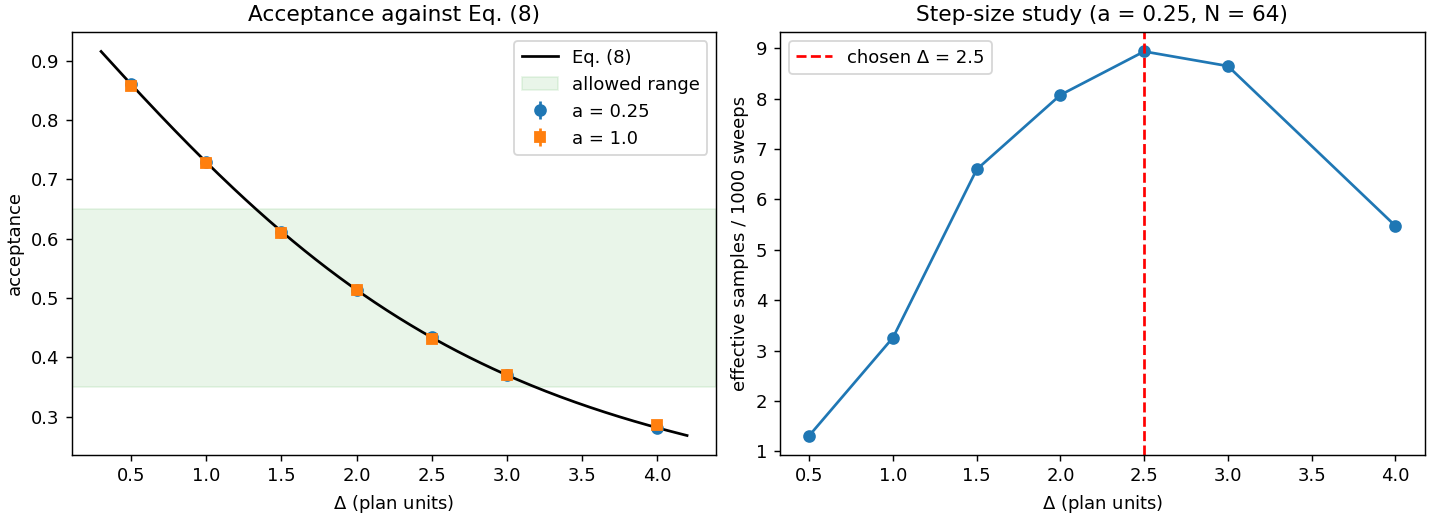
\includegraphics[width=0.95\linewidth]{val_test8_acceptance.png}
\caption{Pilot study for the proposal width (Test 8). Left: measured acceptance
at $a = 0.25$ (circles) and $a = 1$ (squares) against Eq.~\eqref{eq:pacc}; the
shaded band is the allowed range of 35--65\%. Right: effective samples per 1000
sweeps at $a = 0.25$; $\Delta = 2.5$ gives the most.}
\label{fig:tuning}
\end{figure}

The path average $\bar{x}$ changes more slowly than the other observables. It
corresponds to the mode with the smallest eigenvalue, so moving one site at a
time changes it only a little. In the main run, its integrated autocorrelation
time was $\tau_{\mathrm{int}} = 61.8$ sweeps. We calculated it using
$\tau_{\mathrm{int}} = \tfrac12 + \sum_{t \ge 1}\rho(t)$ with the automatic
window $W \ge 6\,\tau_{\mathrm{int}}(W)$. For $x^2$ we obtained $18.5$ sweeps.

For the main Metropolis simulation, we used seed 2026 and ran 48{,}000 sweeps
from the starting path $\mathbf{x} = 0$. We removed the first 8{,}000 sweeps as
burn-in and kept 40{,}000. This gives about 324 independent samples for
$\bar{x}$ and 1{,}081 for $x^2$. For Tests 5, 6, and 7, we ran four more chains
with the same burn-in and number of saved sweeps. Two started at zero, and two
started from random paths with a width five times larger than the expected
distribution. For the wide starts, $x^2$ was initially about 11, while the
expected value is about 0.5. These chains reached the equilibrium range after
32 and 68 sweeps, much sooner than the end of burn-in (Figs.~\ref{fig:traces}
and~\ref{fig:test7}).

\begin{figure}[htbp]
\centering
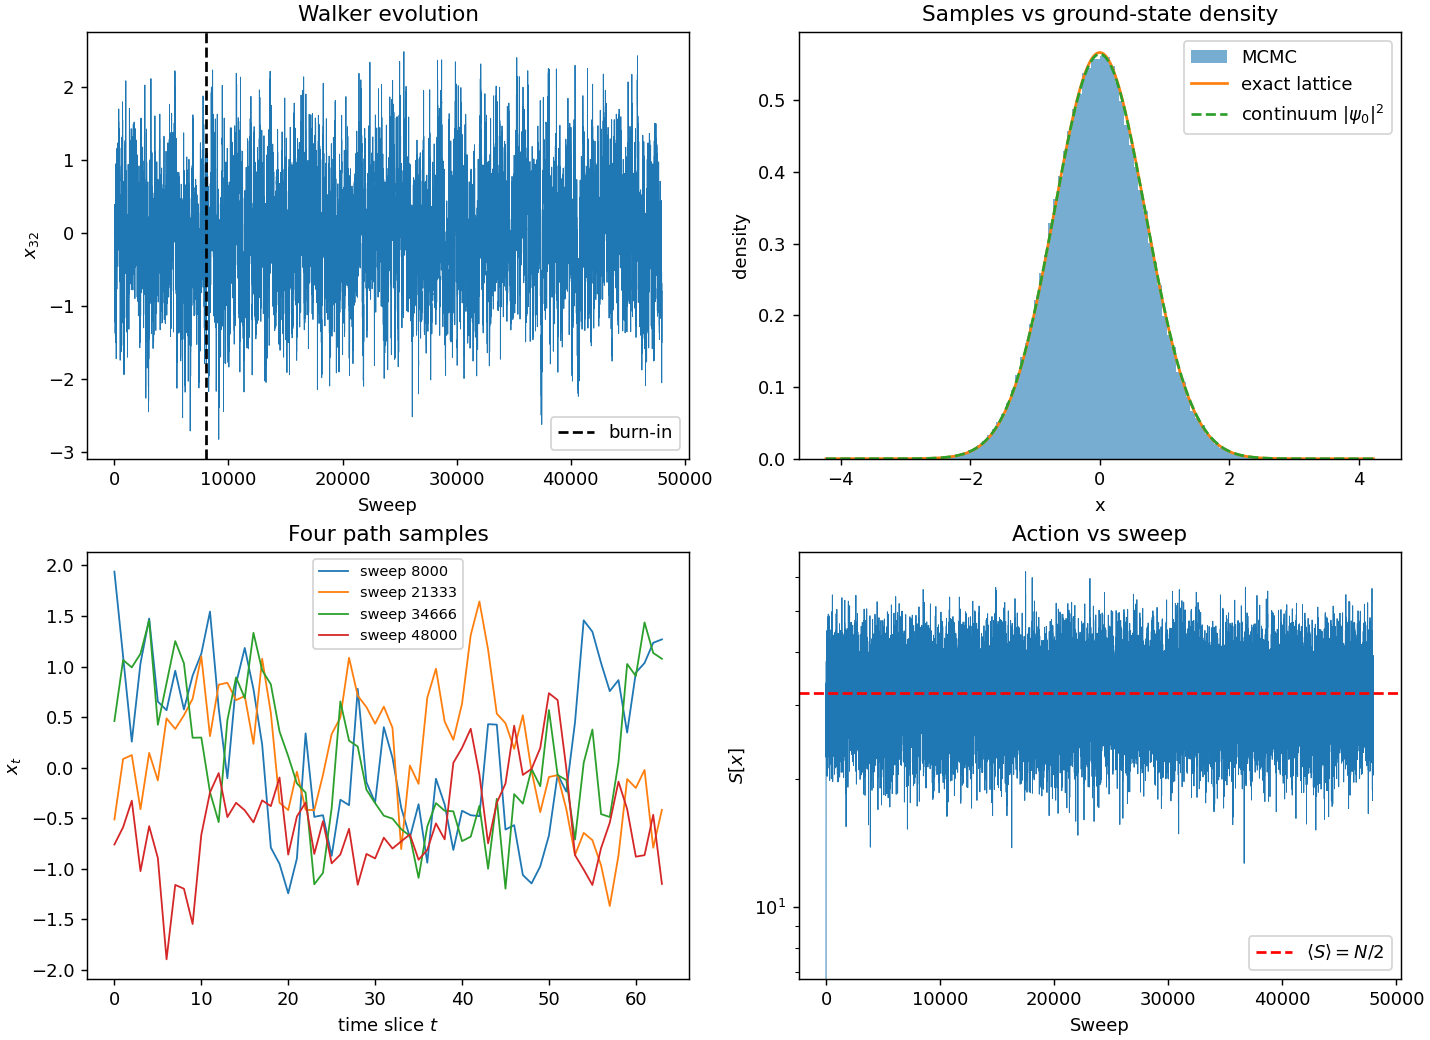
\includegraphics[width=0.85\linewidth]{main_diagnostics.png}
\caption{Diagnostics of the main Metropolis run. Top left: trace of $x_{32}$,
with the end of the burn-in marked. Top right: histogram of all $x_t$ against
the exact lattice Gaussian and the continuum $|\psi_0|^2$. Bottom left: four
sample paths. Bottom right: the action of each sweep, which fluctuates around
$\langle S\rangle = N/2$.}
\label{fig:traces}
\end{figure}

We used 8{,}000 burn-in sweeps, which is much longer than the time needed by
the widest starting paths to reach equilibrium. The 40{,}000 saved sweeps
control the statistical errors. For example, the error of $\langle x\rangle$ is
about $0.015$, and we would need about four times more samples to reduce it by a
factor of two. We kept every sweep because we account for correlations when
calculating errors. Thinning would remove data without giving us more
information.

Neighboring sweeps are correlated, so the usual independent-sample standard
error is not correct. We estimated errors using both binning and the formula
$\sqrt{2\tau_{\mathrm{int}}\,\sigma^2/n}$. In the binning method, we looked for
a stable error using blocks of at least $10\,\tau_{\mathrm{int}}$ and at least
32 blocks. We reported the larger estimate. The code gives a warning if the
binning error does not reach a plateau or if the two error estimates are
different by more than 30\%.

\subsection{Reference Sampler: emcee}

For comparison, we also used the affine-invariant ensemble sampler
\texttt{emcee}~\cite{emcee, goodman}, with the stretch move and
$\log\pi = -S$. We used 128 walkers ($2N$). The walkers started close to zero
with a Gaussian spread of $0.1$. We ran 100{,}000 steps, removed the first
20{,}000 as burn-in, and stored one step out of every 50 to reduce memory. We
calculated the error in two ways: from the spread of the walkers' time
averages, divided by $\sqrt{128}$, and from the time series of the average over
walkers. We used the larger error. The acceptance rate was $0.163$, and the
autocorrelation time of $x^2$ was $357$ steps per walker. Therefore, the
burn-in was about 56 autocorrelation times and the saved part was about 220.
Since adjacent steps are strongly correlated, storing every 50th step loses
little information for this run.

\subsection{Priors}

Priors are omitted since Bayesian parameter fitting is not conducted. The
parameters $m$, $\omega$, $a$, and $N$ are specified before sampling, and the
physical distribution $e^{-S}$ is sampled directly. In Test 10, $m$ and
$\omega$ are estimated from the correlator using least squares, rather than
from a posterior distribution.


\section{Software and Reproducibility}\label{sec:software}

The codebase is structured as an installable Python package,
\texttt{sho-mcmc}. Installation from the repository is accomplished using
\texttt{python3 -m pip install -e .}. Dependencies, as specified in
\texttt{pyproject.toml}, include NumPy, SciPy, Matplotlib, \texttt{emcee}, and
\texttt{tqdm}. The code adheres to PEP~8 style guidelines, applies
\texttt{black} formatting, and employs numpydoc for function documentation.
Sampling operations utilize NumPy arrays. Distinct files are responsible for
managing the action and exact results (\texttt{lattice.py}), Metropolis
sampling (\texttt{metropolis.py}), \texttt{emcee} sampling
(\texttt{ensemble.py}), diagnostics (\texttt{diagnostics.py}), chain
comparisons (\texttt{chains.py}), and physics results (\texttt{verify.py} and
\texttt{plots.py}). Validation tests are implemented in \texttt{checks.py},
\texttt{symmetries.py}, \texttt{convergence.py}, \texttt{tuning.py},
\texttt{injection.py}, \texttt{walkers.py}, and \texttt{multiwalker.py}. Four
principal commands are available:
\begin{itemize}
  \item \texttt{sho-mcmc} runs the main Metropolis chain, and with
    \texttt{-{}-emcee} also \texttt{emcee}, and prints the physics and
    symmetry checks for both (Test 9);
  \item \texttt{sho-mcmc-validate} runs Tests 1--8 and 11;
  \item \texttt{sho-mcmc-inject} runs Test 10;
  \item \texttt{python3 scripts/break\_code.py} runs Test 12.
\end{itemize}
When invoked with \texttt{-{}-out}, each command saves plots, settings, the
random seed, and numerical results. The script \texttt{bash
scripts/run\_all.sh} executes all commands with seed 2026, storing the results
in the \texttt{results/} directory. The process requires approximately 12
minutes on the test system. Pull requests are employed to review changes prior
to merging into the main branch.

\section{Sampling Results}\label{sec:results}

Table~\ref{tab:physics} reports the energy values and symmetry checks obtained
from Metropolis and \texttt{emcee}. All results are within $1.1\sigma$ of the
exact lattice values, and both samplers are consistent with each other within
$1.3\sigma$. The position histograms align with the expected Gaussian
distribution (Fig.~\ref{fig:dist}). Metropolis yields
$\langle x^2\rangle = 0.4995 \pm 0.0045$, closely matching the exact value of
$0.4961$.

For $a = 0.25$, the lattice values differ by approximately 1\% from the
continuum values (Table~\ref{tab:exact}). The extended \texttt{emcee} run
reveals this small difference: its primitive energy is $0.4951 \pm 0.0016$,
which is $0.6\sigma$ from the lattice result but $3.1\sigma$ below the
continuum value of $0.5$. The larger Metropolis error precludes clear
separation of these values.

\subsection*{Symmetries and Degeneracies}

Three symmetries of the distribution were assessed. First, changing $x$ to
$-x$ should not affect the probability, so averages of odd powers must be zero.
Both samplers yield $\langle x\rangle$ and $\langle x^3\rangle$ within
$0.9\sigma$ of zero. The mean at three additional slices also agrees with zero
within $1.5\sigma$ (Test 6). Second, all slices should display the same
distribution due to the periodic structure of the lattice. For
$\langle x_t^2\rangle$, only 2 out of 64 slices in Metropolis and 4 out of 64
in \texttt{emcee} differ from the exact value by more than $2\sigma$,
consistent with expectations from random fluctuations. The first and second
halves of the path, as well as even and odd slices, are consistent. The values
at $t = 0$, $N/4$, $N/2$, and $3N/4$ agree with $C(0)$ within $2.0\sigma$.
Third, time reversal symmetry requires that forward and backward correlators
are equal, and agreement is observed at every separation. In Test 6,
$\langle x_{32}x_{36}\rangle - \langle x_{32}x_{28}\rangle = -0.0042 \pm
0.0071$ was obtained. All main symmetry differences are within $1.3\sigma$
(Fig.~\ref{fig:sympulls}).

\begin{figure}[htbp]
\centering
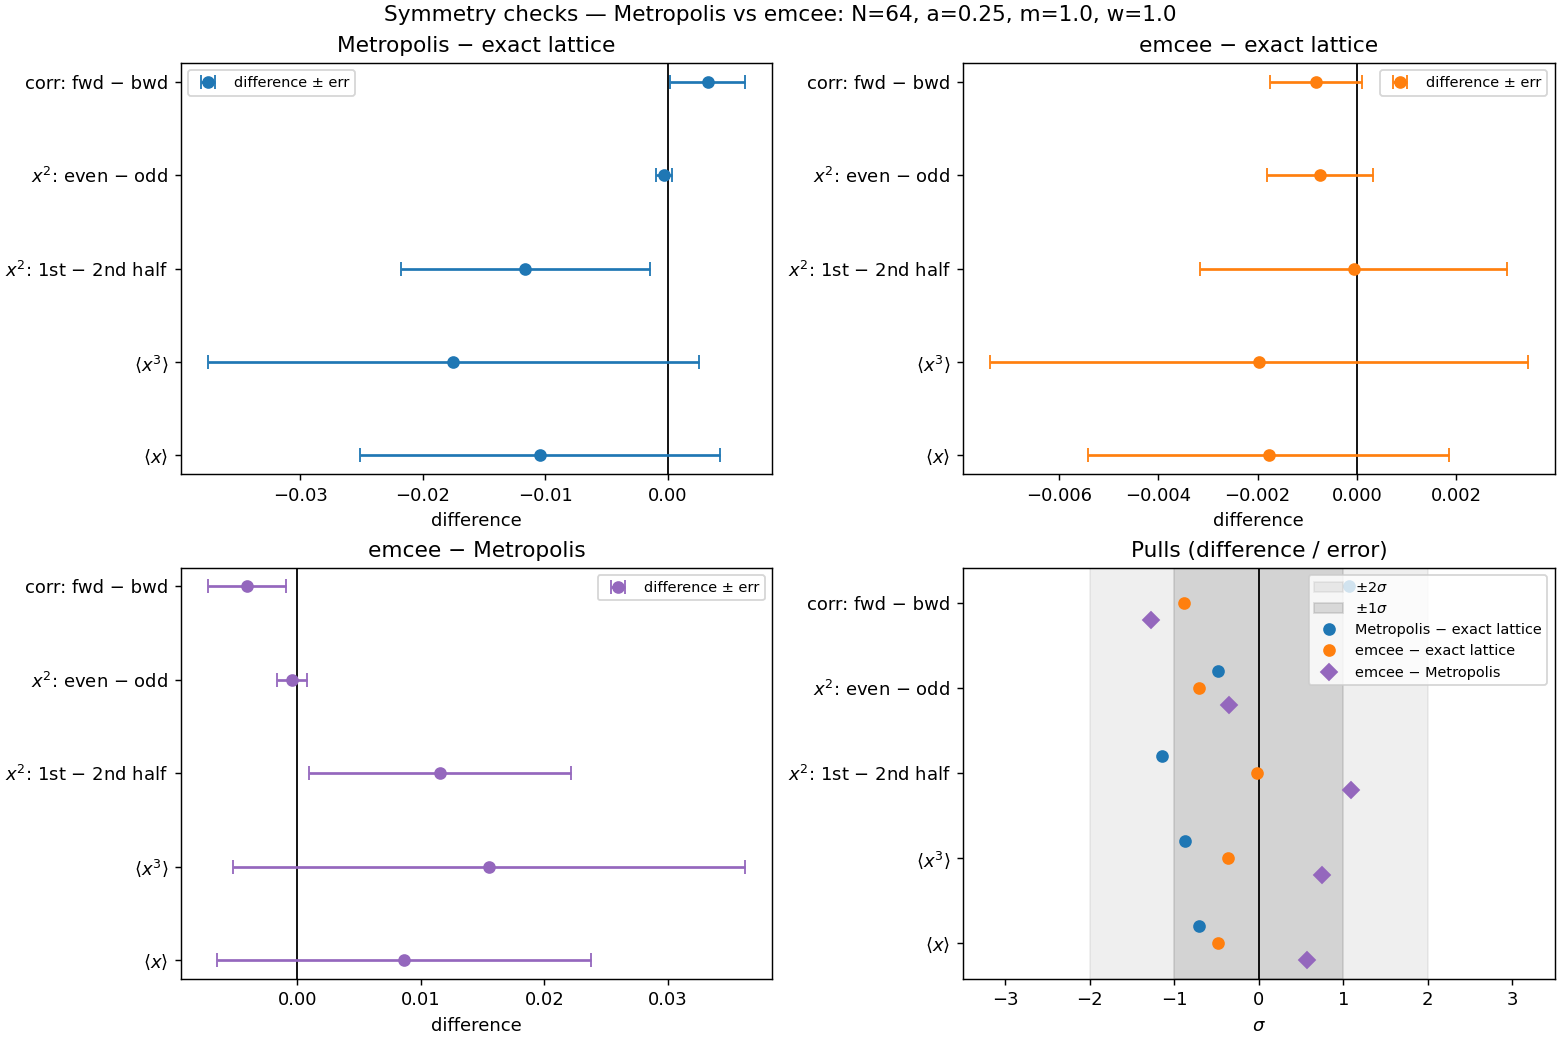
\includegraphics[width=0.85\linewidth]{main_symmetry_pulls.png}
\caption{Symmetry checks in the main run. Top: the results from Metropolis and
\texttt{emcee} compared with zero. Bottom left: difference between the two
samplers. Bottom right: all differences in units of their errors.}
\label{fig:sympulls}
\end{figure}

The matrix $K$ is positive definite, resulting in a target distribution with a
single peak at $\mathbf{x} = 0$. Chains initialized from zero and from wide
random paths converge to the same final distribution, with
$\langle x^2\rangle$ and $C(4)$ agreeing within $0.6\sigma$. In Test 10,
$\omega$ and $-\omega$ yield the same action because only $\omega^2$ appears;
therefore, $\omega > 0$ is used. With this convention, the input frequency is
recovered within $2.1\sigma$ on all five lattices.

\begin{table}[htbp]
\centering
\small
\begin{tabular}{lccccc}
\toprule
 & Metropolis & & \texttt{emcee} & & \texttt{emcee} $-$ Metr.\\
\midrule
$\langle V\rangle$ & $0.2497 \pm 0.0026$ & $+0.6\sigma$ & $0.2474 \pm 0.0010$ & $-0.7\sigma$ & $-0.8\sigma$\\
$\langle T\rangle$ (primitive) & $0.2470 \pm 0.0035$ & $-0.3\sigma$ & $0.2477 \pm 0.0011$ & $-0.3\sigma$ & $+0.2\sigma$\\
$E$ (primitive) & $0.4967 \pm 0.0035$ & $+0.2\sigma$ & $0.4951 \pm 0.0016$ & $-0.6\sigma$ & $-0.4\sigma$\\
$E$ (virial) & $0.4995 \pm 0.0053$ & $+0.6\sigma$ & $0.4948 \pm 0.0019$ & $-0.7\sigma$ & $-0.8\sigma$\\
\midrule
$\langle x\rangle$ & $-0.0104 \pm 0.0147$ & $-0.7\sigma$ & $-0.0018 \pm 0.0036$ & $-0.5\sigma$ & $+0.6\sigma$\\
$\langle x^3\rangle$ & $-0.0175 \pm 0.0200$ & $-0.9\sigma$ & $-0.0020 \pm 0.0054$ & $-0.4\sigma$ & $+0.7\sigma$\\
$x^2$: first $-$ second half & $-0.0116 \pm 0.0102$ & $-1.1\sigma$ & $-0.0001 \pm 0.0031$ & $-0.0\sigma$ & $+1.1\sigma$\\
$x^2$: even $-$ odd slices & $-0.0003 \pm 0.0006$ & $-0.5\sigma$ & $-0.0007 \pm 0.0011$ & $-0.7\sigma$ & $-0.4\sigma$\\
$C$: forward $-$ backward & $+0.0033 \pm 0.0031$ & $+1.1\sigma$ & $-0.0008 \pm 0.0009$ & $-0.9\sigma$ & $-1.3\sigma$\\
\bottomrule
\end{tabular}
\caption{Energies (top) and symmetry checks (bottom) of the main run, with the
pull against the exact lattice value (Table~\ref{tab:exact}; zero for every
symmetry check) and the difference between the samplers in units of the
combined error.}
\label{tab:physics}
\end{table}

\begin{figure}[htbp]
\centering
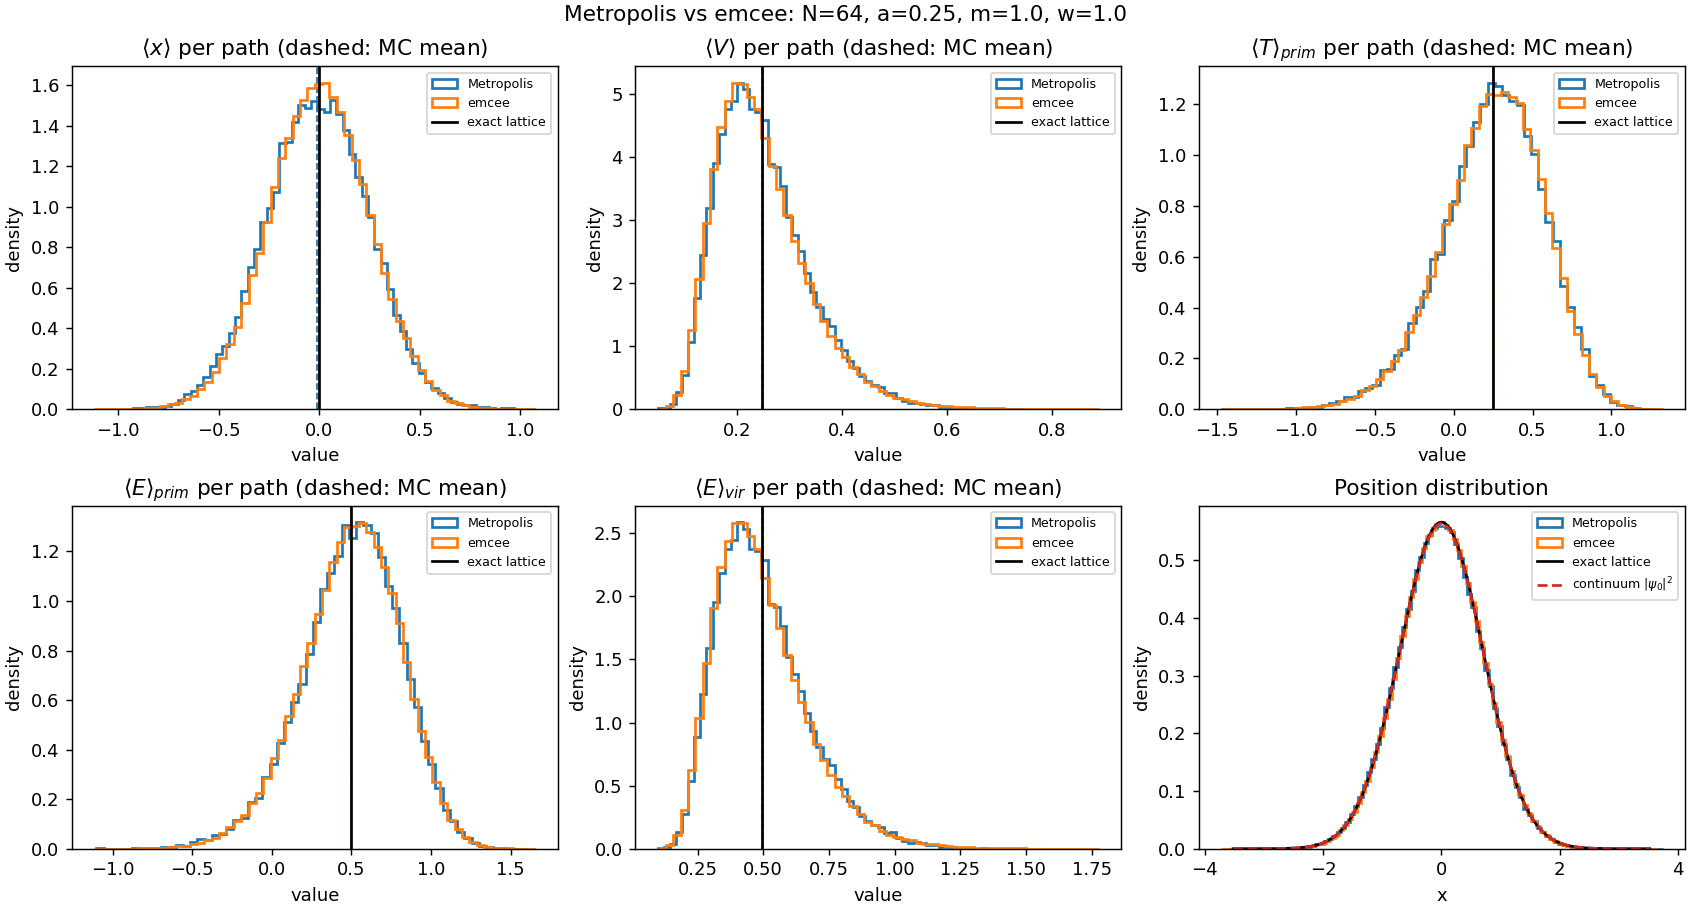
\includegraphics[width=\linewidth]{main_distributions.png}
\caption{Distributions of the per-path averages of $x$, the potential, kinetic
and total energies, and of all positions $x_t$, for Metropolis and
\texttt{emcee}, with the exact lattice values.}
\label{fig:dist}
\end{figure}


\section{Convergence}\label{sec:convergence}

We checked convergence using four methods.

\paragraph{Multiple-chain diagnostics (Test 7).} We used four chains with
different starting paths. For nine quantities, we calculated the
rank-normalized split $\hat R$~\cite{vehtari, gelman} and the effective sample
size (ESS). The largest $\hat R$ was $1.0037$, below our limit of $1.01$, and
the smallest ESS was 1342, above our limit of 400. The path average had the
slowest mixing. We also tested the $\hat R$ calculation itself: four similar
chains gave $1.0001$, while shifting one chain by half a standard deviation
increased it to $1.0232$.

\paragraph{Autocorrelation and binning.} The autocorrelation of $x^2$
decreases to about zero within 100 sweeps. The automatic window was $W = 112$,
giving $\tau_{\mathrm{int}} = 18.5$ sweeps (Fig.~\ref{fig:autocorr}). In the
binning plot, the error of $\langle x^2\rangle$ becomes stable near $0.0045$
for blocks longer than about 100 sweeps (Fig.~\ref{fig:binning}). These results
demonstrate the necessity of accounting for correlations between samples.
Error calculations were validated using AR(1) data with known results. The
autocorrelation time was within 1.3\% and the binning error within 5\% of the
expected values.

\paragraph{Trace plots.} Figure~\ref{fig:test7} displays all four chains. Even
chains initialized with wide starting paths reached the equilibrium range
within approximately 70 sweeps. Subsequently, the chains explored the same
region, and no systematic drift was observed.

\paragraph{Multiple walkers (Test 11).} We ran eight walkers with two types of
starting conditions. For a Gaussian, the expected probability of being within
one standard deviation is $\mathrm{erf}(1/\sqrt2) = 0.6827$. We measured this
fraction for the middle slice and the path average. Each walker agreed with the
exact fraction within $2.0\sigma$ (Fig.~\ref{fig:walkers}). Comparing the
walkers gave $\chi^2 = 9.2$ and $3.6$ with 7 degrees of freedom ($p = 0.24$ and
$0.82$). In Alex's first version of the test, six walkers used $N = 100$
and $a = 0.5$. Their $\langle x^2\rangle$ and time spent in five regions
matched the exact results within $0.4\sigma$, with $\hat R \le 1.0003$.

\begin{figure}[htbp]
\centering
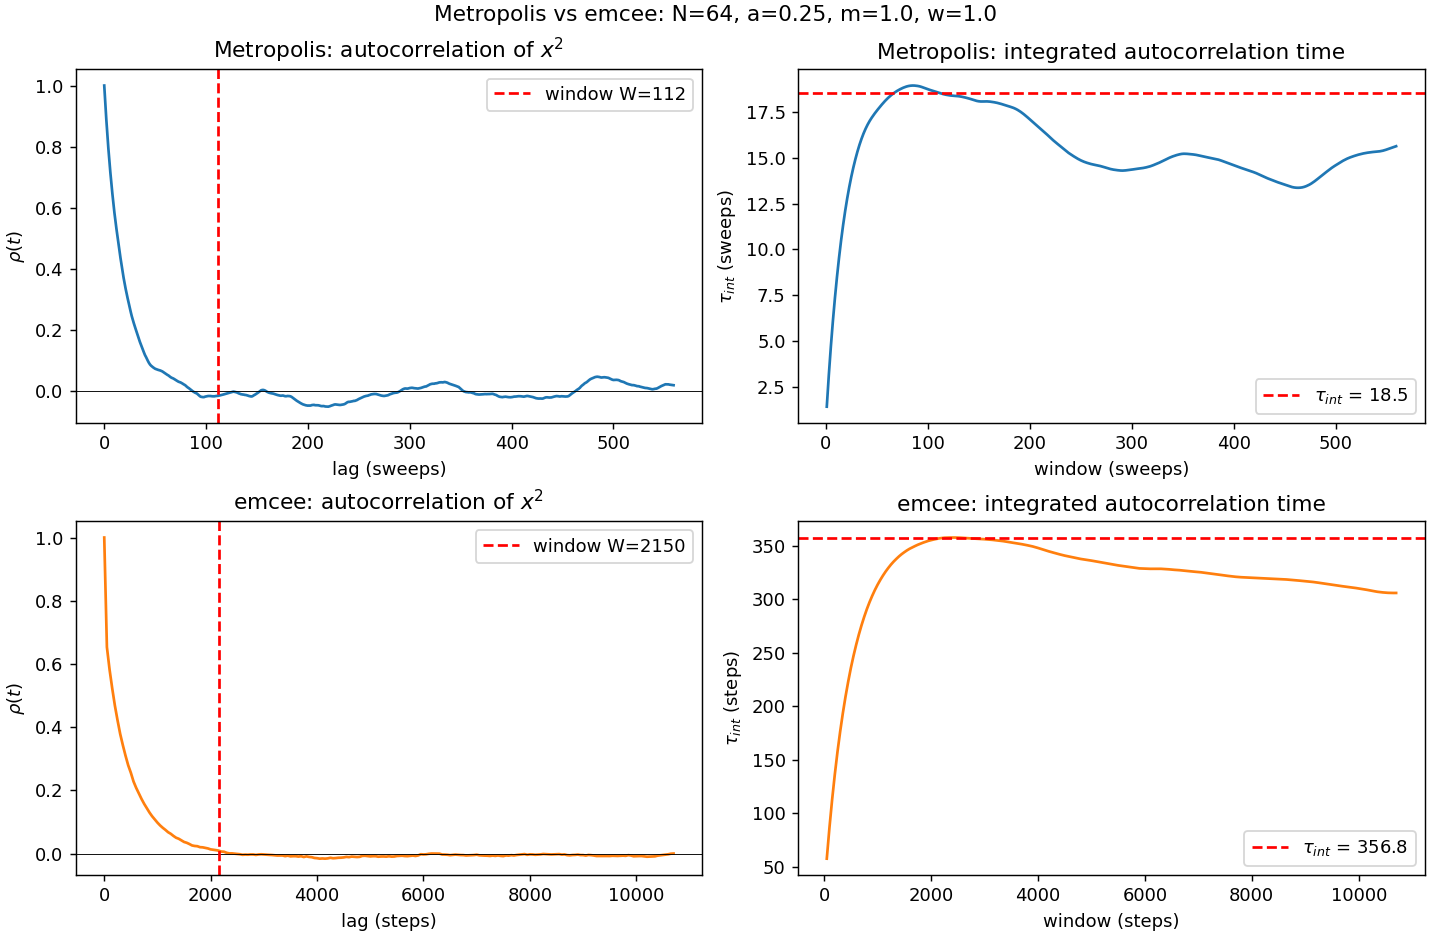
\includegraphics[width=0.85\linewidth]{main_autocorr.png}
\caption{Autocorrelation of $x^2$ (left) and integrated autocorrelation time
against the summation window (right), for Metropolis in sweeps (top) and for
\texttt{emcee} in steps (bottom). The dashed lines mark the automatic window
and the resulting $\tau_{\mathrm{int}}$.}
\label{fig:autocorr}
\end{figure}

\begin{figure}[htbp]
\centering
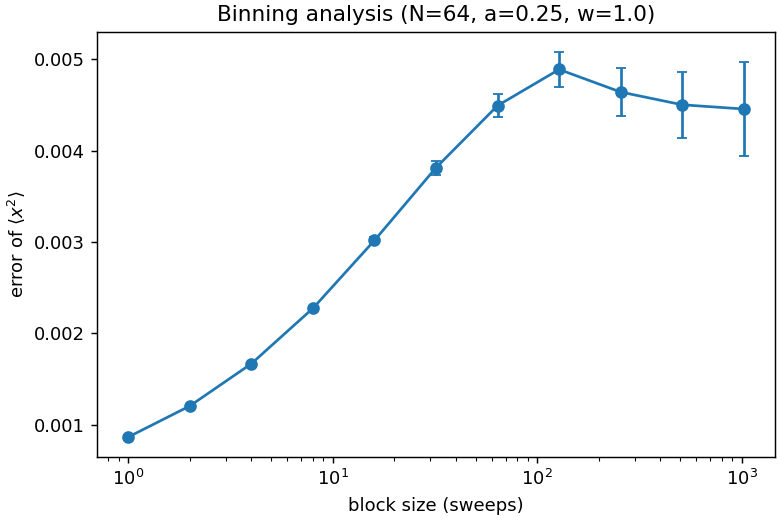
\includegraphics[width=0.55\linewidth]{main_binning.png}
\caption{Binning analysis of $\langle x^2\rangle$ in the main Metropolis run.
The error reaches a plateau of about $0.0045$ for blocks longer than about 100
sweeps.}
\label{fig:binning}
\end{figure}

\begin{figure}[htbp]
\centering
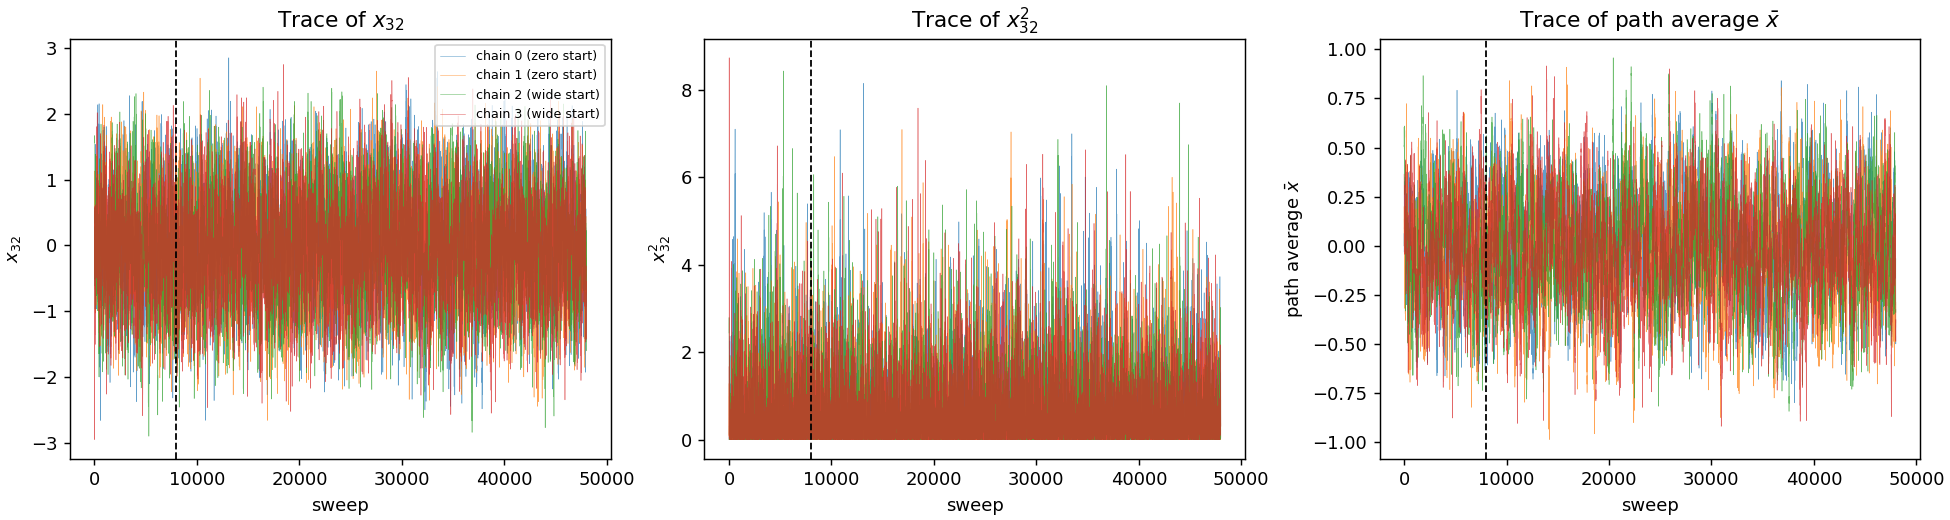
\includegraphics[width=\linewidth]{val_test7_traces.png}
\caption{Trace plots of the four chains of Test 7: $x_{32}$, $x_{32}^2$ and the
path average, with the end of the burn-in marked by the dashed line.}
\label{fig:test7}
\end{figure}

\begin{figure}[htbp]
\centering
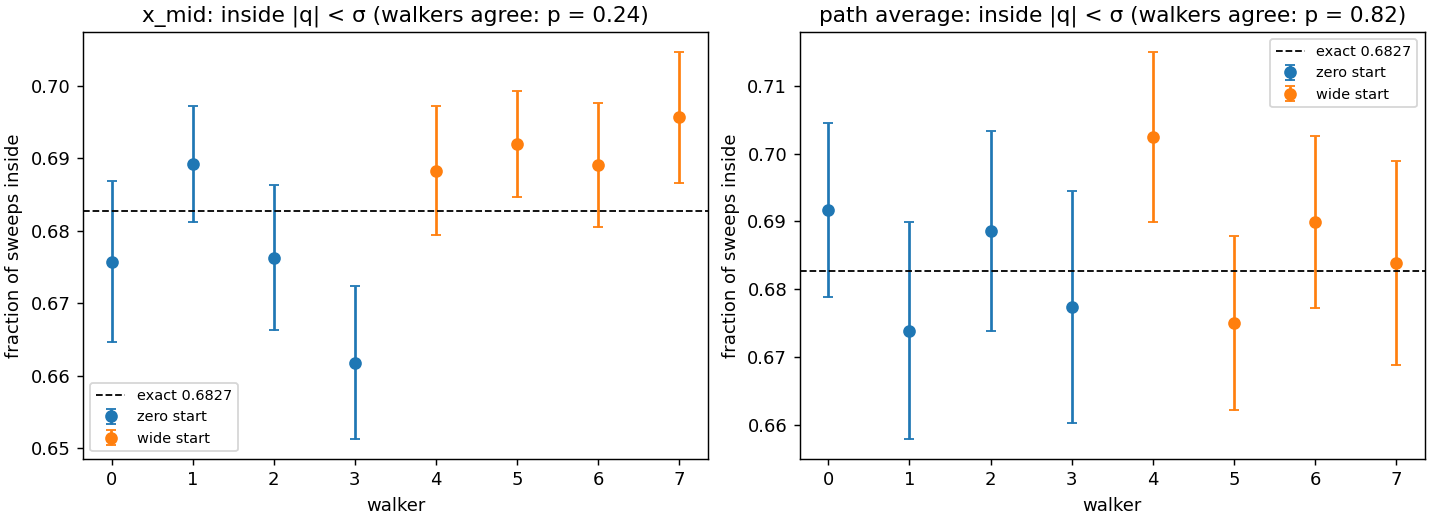
\includegraphics[width=0.9\linewidth]{val_test11_walkers.png}
\caption{Test 11: fraction of sweeps that each walker spends inside one
standard deviation, for $x$ at the middle slice (left) and for the path average
(right), against the exact fraction 0.6827.}
\label{fig:walkers}
\end{figure}


\section{Comparison of Metropolis and emcee}\label{sec:emcee}

Metropolis and \texttt{emcee} produced consistent results for the oscillator
(Table~\ref{tab:physics} and Fig.~\ref{fig:comparison}). Only 2 out of 64
Metropolis values and 4 out of 64 \texttt{emcee} values for
$\langle x_t^2\rangle$ deviated by more than $2\sigma$ from the exact answer.
The correlators and the forward-minus-backward differences were all within
$2\sigma$ (Fig.~\ref{fig:symmetries}). The virial check
$\langle T\rangle - \langle V\rangle$, which should be zero, was
$-0.0028 \pm 0.0048$ for Metropolis and $+0.0003 \pm 0.0009$ for
\texttt{emcee}.

The primary distinction was computational cost. Metropolis required
approximately 1.1 seconds for 48{,}000 sweeps and yielded about 1{,}081
independent samples of $x^2$. The \texttt{emcee} run required around 21 seconds
for 100{,}000 steps of 128 walkers and produced approximately 14{,}351
independent samples. This corresponds to about 1{,}000 effective samples per
second for Metropolis and 700 for \texttt{emcee}. A single \texttt{emcee}
walker progressed more slowly: its acceptance rate was $0.163$ and its
autocorrelation time was 357 steps, compared with 18.5 sweeps for Metropolis.
This difference arises because the stretch move updates all 64 coordinates
simultaneously. The single-site method leverages the fact that each site
interacts only with neighboring sites, and the checkerboard update is
efficient with NumPy.

\begin{figure}[htbp]
\centering
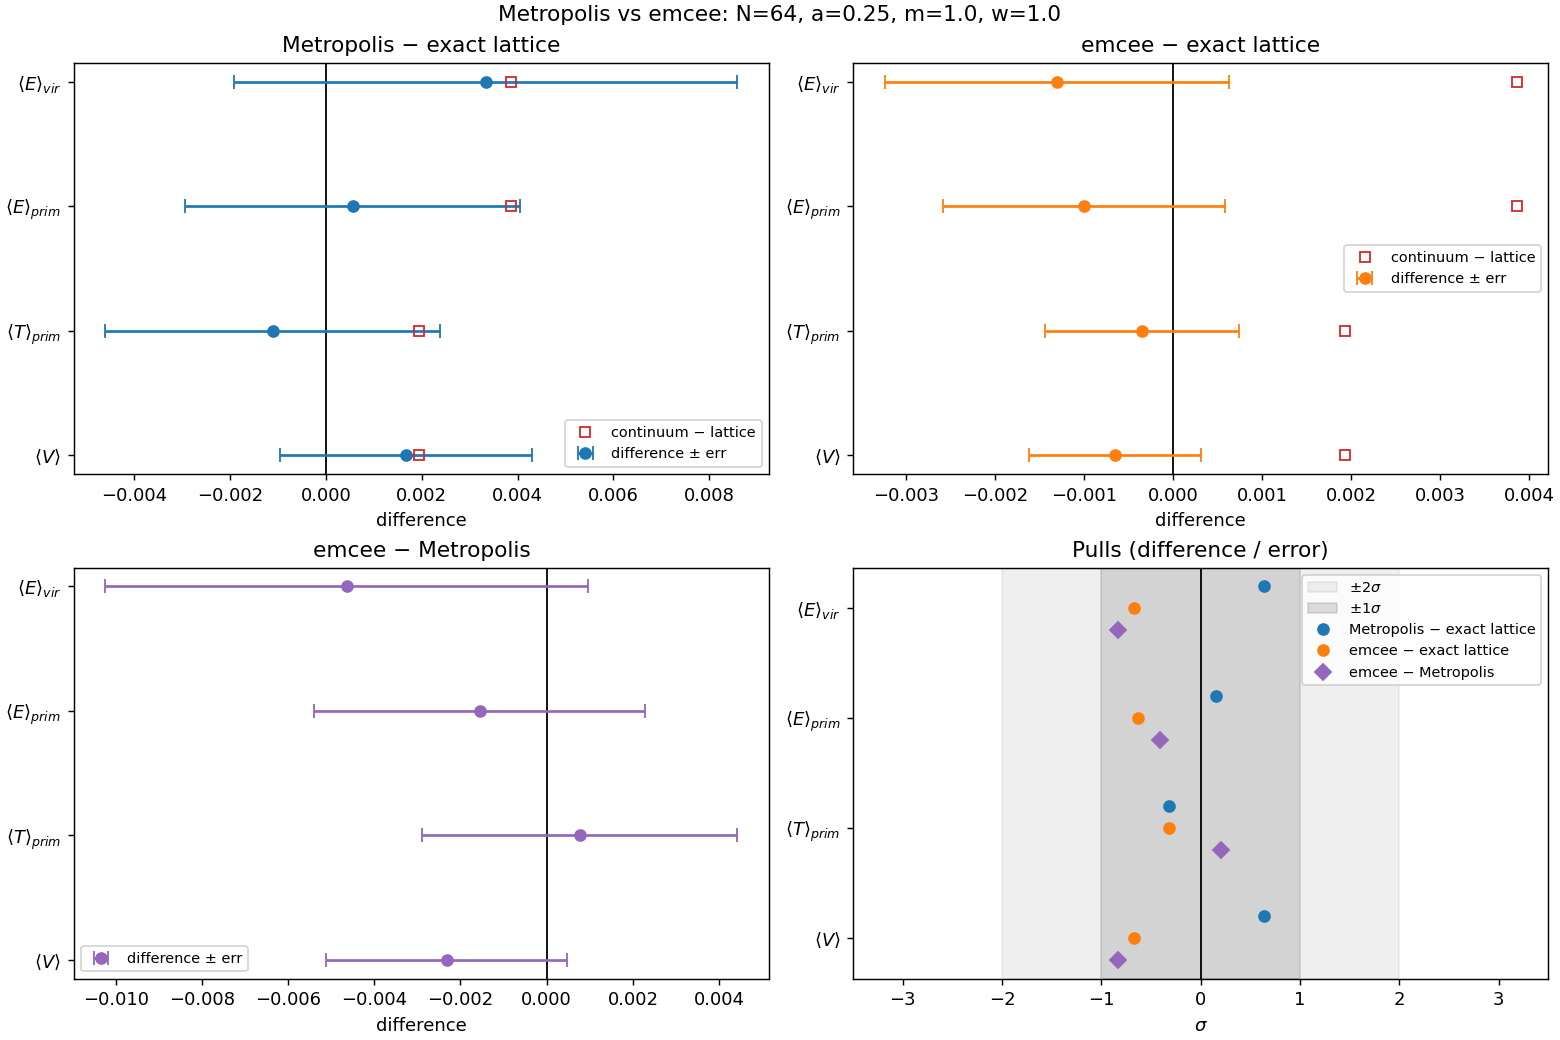
\includegraphics[width=0.85\linewidth]{main_comparison.png}
\caption{Energies of Metropolis and \texttt{emcee} against the exact lattice
values (top), against each other (bottom left), and all pulls (bottom right).
The squares show how far the continuum lies from the lattice value.}
\label{fig:comparison}
\end{figure}

\begin{figure}[htbp]
\centering
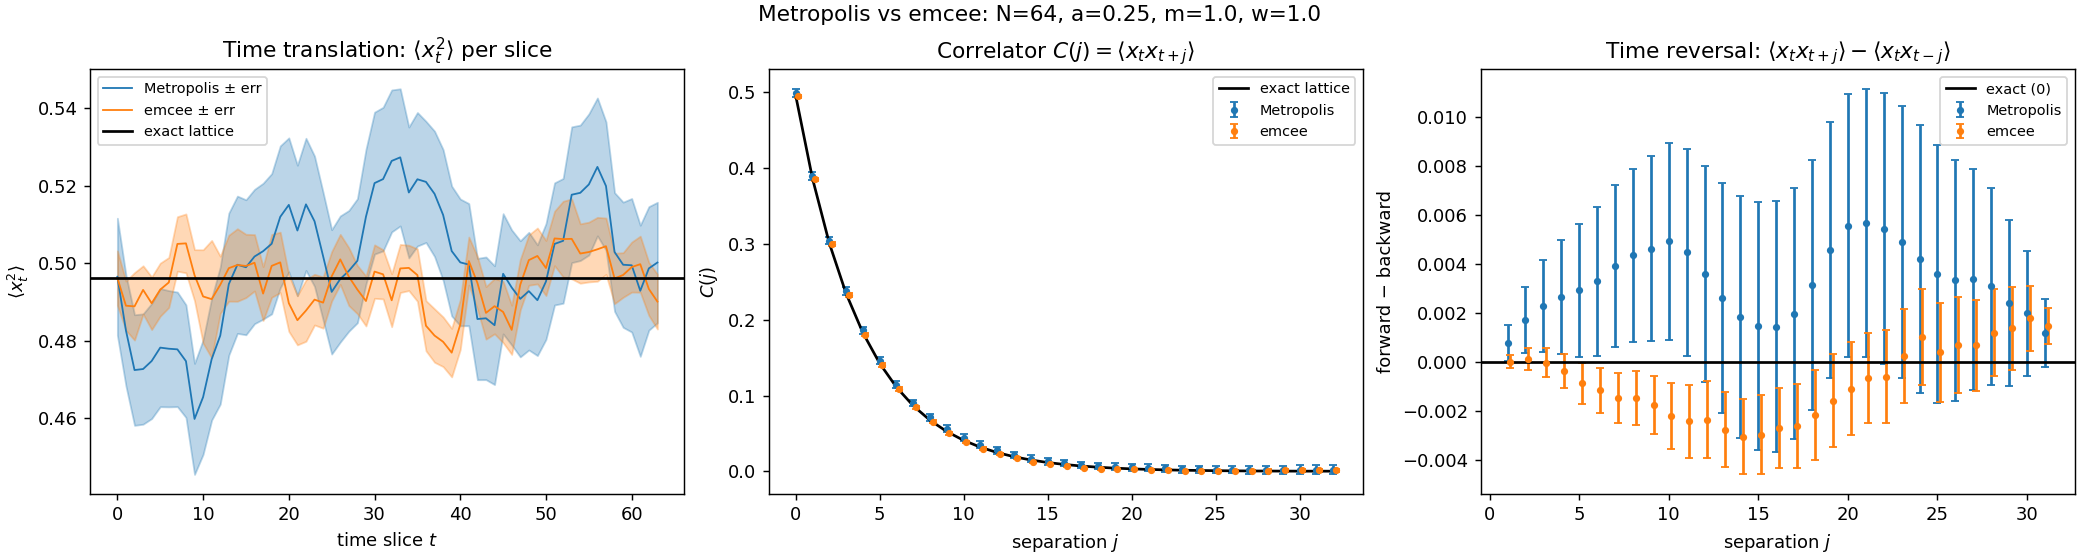
\includegraphics[width=\linewidth]{main_symmetries.png}
\caption{Left: $\langle x_t^2\rangle$ at every slice (time translation). Middle:
the correlator $C(j)$ against Eq.~\eqref{eq:corr}. Right: forward minus
backward correlator (time reversal), which must be zero.}
\label{fig:symmetries}
\end{figure}


\section{Validation}\label{sec:validation}

The initial validation plan was prepared prior to code development. It was
subsequently updated during implementation and result verification. The
repository contains all plan versions, from \texttt{Validation\_V1.tex} to
\texttt{Validation\_V1.5.tex}, as well as \texttt{Validation.pdf}. The original
LaTeX file was committed on November 14 (commit e0529f1), enabling comparison
of changes in Git. For v1.3 and v1.5, a copy of the previous version was saved
before edits were committed. Version v1.4 was committed in a single step.
Table~\ref{tab:versions} provides the version dates, commit IDs, and main
changes.

\subsection{What each test showed}

Table~\ref{tab:results} details, for each test, the execution method and
outcomes from our final run of \texttt{scripts/run\_all.sh} (seed 2026).

\begin{table}[htbp]
\centering
\footnotesize
\setlength{\tabcolsep}{3pt}
\begin{tabular}{p{2.7cm}p{3.0cm}p{5.6cm}}
\toprule
Test & Run with & Result\\
\midrule
1. Action and $\Delta S$ & \texttt{sho-mcmc-validate} & Passed: largest
differences $1.3\times10^{-13}$ and $1.1\times10^{-13}$ (limit $10^{-10}$); both
sweeps give identical chains.\\
2. Exact covariance & \texttt{sho-mcmc-validate} & Passed: eigenvalues within
$8.9\times10^{-15}$, closed form within $2.2\times10^{-16}$.\\
3. Error-bar code & \texttt{sho-mcmc-validate} & Passed: $\tau_{\mathrm{int}}$
within 1.3\% and errors within 5.0\%; $\hat{R}$ rises from 1.0001 to 1.0232 for
the shifted chain.\\
4. Smallest lattice, $N = 2$ & \texttt{sho-mcmc-validate} & Passed: KS
$p = 0.716$ and $0.409$; all moments within $0.5\sigma$, acceptance
$-2.1\sigma$.\\
5. Known answers & \texttt{sho-mcmc-validate} & Passed: all eleven values of
Table~\ref{tab:exact} within $1.3\sigma$.\\
6. Symmetries & \texttt{sho-mcmc-validate} & Passed: all checks within
$2.0\sigma$; the two kinds of start agree within $0.6\sigma$.\\
7. Convergence & \texttt{sho-mcmc-validate} & Passed: $\hat{R} \le 1.0037$,
ESS $\ge 1342$.\\
8. Acceptance and step size & \texttt{sho-mcmc-validate} & Passed: all fourteen
acceptances within $2.1\sigma$ of Eq.~\eqref{eq:pacc}; best $\Delta = 2.5$.\\
9. Metropolis vs \texttt{emcee} & \texttt{sho-mcmc -{}-emcee} & Passed: both
within $1.1\sigma$ of the exact values and within $1.3\sigma$ of each other.\\
10. Injection & \texttt{sho-mcmc-inject} & Passed: all five lattices within
$2.1\sigma$, fit $p$ from 0.42 to 0.78; negative control rejected at
$+9.7\sigma$.\\
11. Multi-walker & \texttt{sho-mcmc-validate} & Passed: every walker within
$2.0\sigma$; walkers agree, $p = 0.24$ and $0.82$.\\
 & \texttt{multiwalker.py} & All walkers within $0.4\sigma$ of the exact
values; $\hat{R} \le 1.0003$.\\
12. Bugs on purpose & \texttt{break\_code.py} & Passed: all six bugs caught.\\
\bottomrule
\end{tabular}
\caption{What each test showed. Commands from our package; settings and
seeds in \texttt{scripts/run\_all.sh}; full output in \texttt{results/}.}
\label{tab:results}
\end{table}

On the smallest lattice (Test 4), the sampled distributions of $x_0 + x_1$ and
$x_0 - x_1$ correspond to the exact Gaussians with variances 2 and 0.4
(Fig.~\ref{fig:test4}).

\begin{figure}[htbp]
\centering
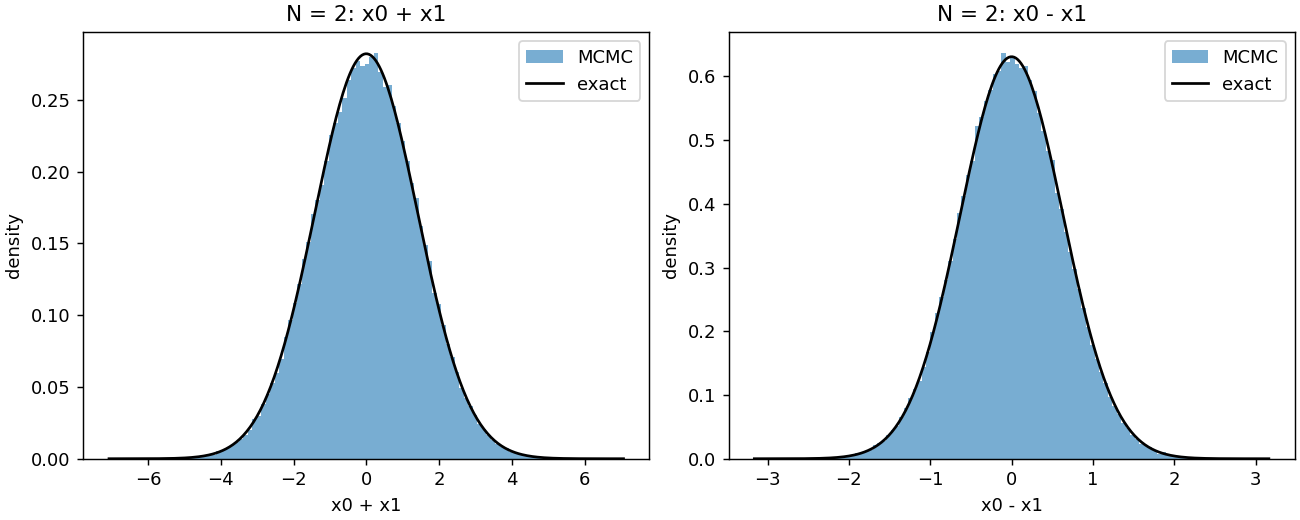
\includegraphics[width=0.8\linewidth]{val_test4_small_lattice.png}
\caption{Test 4 on the $N = 2$ lattice at $a = 1$: histograms of $x_0 + x_1$
and $x_0 - x_1$ from 200{,}000 sweeps against the exact Gaussians.}
\label{fig:test4}
\end{figure}

The injection test (Fig.~\ref{fig:inj}) successfully recovers both input
parameters across all five lattices, including those with $m \ne 1$ and
$\omega \ne 1$. The measured energy gaps also demonstrate the discretization
effect described in Section~\ref{sec:model}: at $a\omega = 1$, the measured gap
is $0.972 \pm 0.011$ in units of $\omega$, compared to the lattice value
$0.962$ and the continuum value 1. We also verified the reliability of
Test 10's error bars: during development, each of the five lattices was run 24
times with different seeds (120 fits). The pulls had means of $-0.20$ and
$+0.14$ and spreads of $0.97$ and $1.03$ for $m$ and $\omega$, respectively,
closely matching the expected values of 0 and 1 for reliable error bars. Only
one fit in 120 had $p < 10^{-3}$. This procedure can be repeated using
\texttt{sho-mcmc-inject} with the \texttt{-{}-repeats 24} option.

\begin{figure}[htbp]
\centering
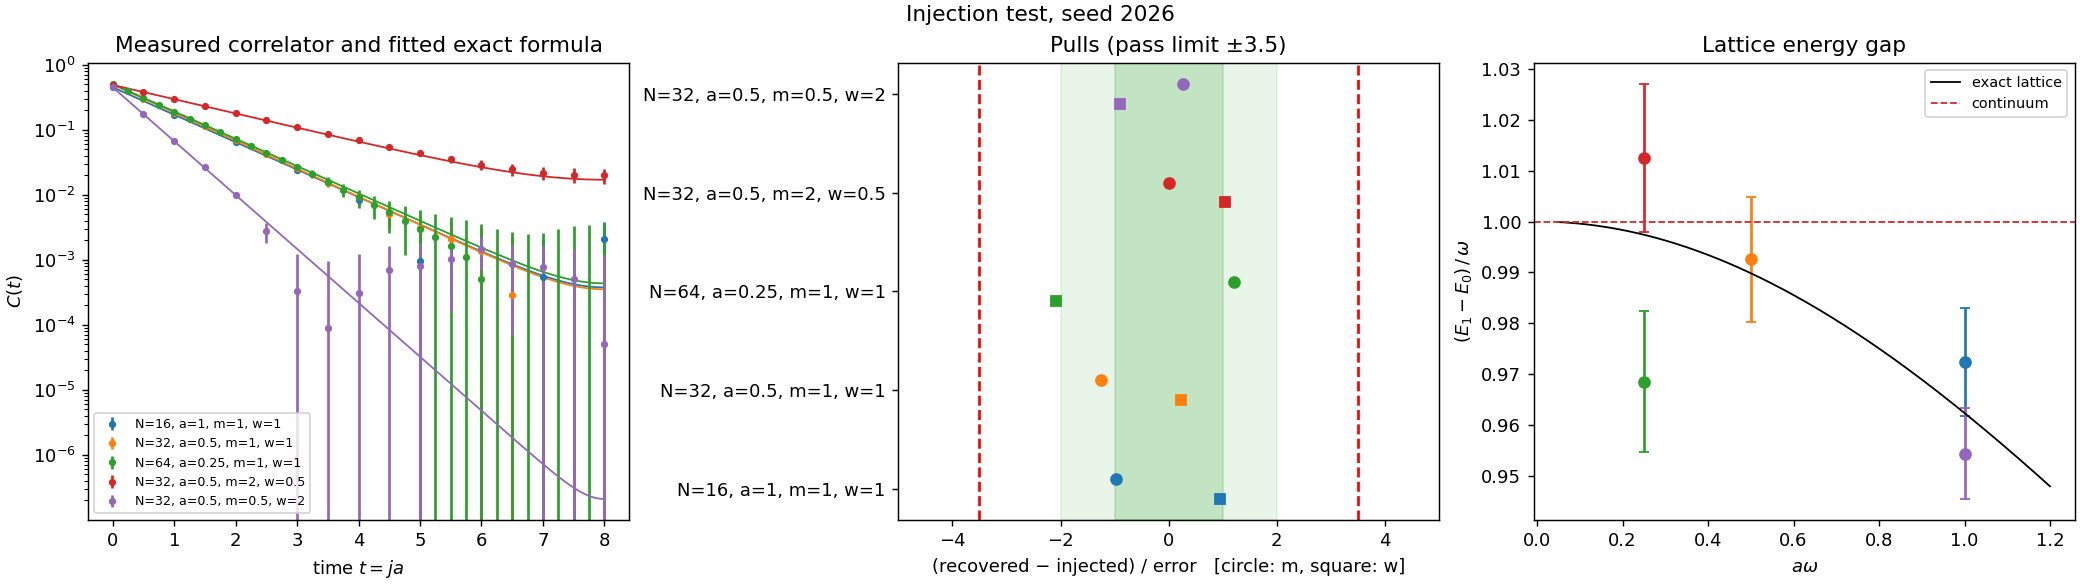
\includegraphics[width=\linewidth]{inj.png}
\caption{Injection test (Test 10). Left: measured correlators of the five
lattices with the fitted exact formula. Middle: pulls of the recovered $m$
(circles) and $\omega$ (squares); the dashed lines are the pass limits
$\pm3.5$. Right: measured energy gap against the lattice formula and the
continuum.}
\label{fig:inj}
\end{figure}

\subsection{What the Testing Caught}

{\sloppy
\begin{itemize}
\item \textbf{The code and the initial plan described different models.} The
  code samples a periodic lattice with the potential evaluated at the slices,
  whereas v1 assumed fixed endpoints and excluded periodic boundaries. No test
  detected this discrepancy because the code's exact results were calculated
  for the same periodic lattice as the sampler, resulting in agreement between
  the two, despite both differing from the plan. This difference was identified
  while verifying the exact correlator required for Test 10. The plan
  (v1.2--v1.4) was updated to clarify the use of the periodic lattice in the
  simulations. A periodic lattice yields the thermal distribution at
  temperature $1/T$. For $\omega T = 16$, the deviation from the ground state is
  negligible, approximately $e^{-16}$. The periodic version also exhibits
  time-shift symmetry, which was tested in Test 6.
\item \textbf{$N = 3$ cannot be executed.} The checkerboard update requires an
  even $N$, so the $N = 3$ portion of Test 4 was not feasible. This was
  discovered during the revision of Test 4, and only $N = 2$ was retained.
\item \textbf{Step sizes are expressed in different units.} The plan's
  acceptance formula uses $\Delta$, while the code uses $\delta$. Conversion is
  performed using $\delta = \Delta/\sqrt{A}$, which resulted in the measured
  acceptance matching Eq.~\eqref{eq:pacc} at both lattice spacings (Test 8),
  thereby confirming the validity of the conversion.
\item \textbf{Bugs introduced intentionally (Test 12).} Six bugs were inserted
  into a temporary copy of the code, one at a time, and each resulted in at
  least one test failure, as anticipated by the testing plan. Issues such as
  retaining rejected steps, an incorrect sign in $\Delta S$, an incorrect
  neighbor, and updating all sites simultaneously were each detected by Test 1
  and several statistical tests. Error bars that neglected autocorrelation were
  identified only by Test 3. A missing factor $m$ in the potential was detected
  exclusively by Test 10: for cases with $m \ne 1$, the code's exact
  $\langle x^2\rangle$ no longer matched the formula from the action, causing
  the test to halt with an error. When $m = 1$, no other test could detect this
  bug, which is why Test 10 includes cases with $m \ne 1$.
\item \textbf{A script was disrupted by an external change.} During the review
  of Alex's pull request, the multi-walker script failed at an import
  because the package had relocated \texttt{verify\_sho.py}. After updating the
  import and adding a fixed seed, the script executed successfully and produced
  results consistent with the exact values.
\item \textbf{Mistakes in the workflow.} Initially, the package files did not
  exclude build files generated by \texttt{pip install -e .}
  (\texttt{*.egg-info}), resulting in their accidental inclusion in the
  repository. These files were subsequently removed, and tracking of an
  outdated \texttt{\_\_pycache\_\_} folder was discontinued. An early update for
  Tests 1--5 and 7 inadvertently used an older, unformatted version of the
  package. This issue was identified during file
  comparisons, as applying the update would have altered the formatting of 15
  files. The current files were used to resolve this. Later, copying with
  Finder replaced the entire \texttt{src} folder and deleted many package files
  on one computer. Running \texttt{git status} before committing revealed this,
  allowing restoration of the files from Git.
\end{itemize}
\par}

\section{Use of Artificial Intelligence}

Artificial intelligence was used to write the original script for the \texttt{multiwalker.py} test and add the docstrings according to numpy format. 

\section{Discussion and conclusions}

The Metropolis sampler and \texttt{emcee} both produced results consistent with
the exact lattice distribution. The energies, correlators, position histograms,
and symmetry checks all agree within their statistical errors. The four
Metropolis chains have $\hat R \le 1.0037$, and the binning analysis indicates
stable error estimates. The multi-walker test also aligns with the Gaussian
expectation. In Test 10, the fitted mass and frequency match the known input
values, and the wrong-frequency control was rejected at $9.7\sigma$. All final
tests were successful.

An important lesson was that the original plan and the first implementation
were based on different boundary conditions. The numerical checks did not
reveal this discrepancy, as both the implementation and its exact reference
values used the same periodic lattice. It was necessary to compare the plan
with the model implemented in the code. Test 12 was valuable in demonstrating
whether the checks could detect incorrect implementations. All six introduced
bugs were identified. Specifically, the missing factor of $m$ was detected only
in Test 10, since that test includes cases with $m \ne 1$.

Some limitations remain. Most of the analysis was conducted using a single
lattice with $N = 64$ and $a = 0.25$. Only one extended \texttt{emcee} run was
performed, rather than several independent runs. The path average is the
slowest observable and yielded approximately 324 effective samples in the main
Metropolis run. Floating-point warnings were observed on macOS for matrix
calculations in Test 1, although the numerical difference was only
$1.1\times10^{-13}$. For much larger lattices or smaller spacing, local updates
may become less efficient, and more collective proposals could be beneficial.


\begin{thebibliography}{9}
\bibitem{creutz} M. Creutz and B. Freedman, ``A statistical approach to quantum
mechanics,'' Annals of Physics \textbf{132}, 427 (1981).
\bibitem{metropolis} N. Metropolis, A. W. Rosenbluth, M. N. Rosenbluth,
A. H. Teller and E. Teller, ``Equation of state calculations by fast computing
machines,'' J. Chem. Phys. \textbf{21}, 1087 (1953).
\bibitem{emcee} D. Foreman-Mackey, D. W. Hogg, D. Lang and J. Goodman,
``emcee: The MCMC Hammer,'' PASP \textbf{125}, 306 (2013).
\bibitem{goodman} J. Goodman and J. Weare, ``Ensemble samplers with affine
invariance,'' Commun. Appl. Math. Comput. Sci. \textbf{5}, 65 (2010).
\bibitem{gelman} A. Gelman and D. B. Rubin, ``Inference from iterative
simulation using multiple sequences,'' Statistical Science \textbf{7}, 457
(1992).
\bibitem{vehtari} A. Vehtari, A. Gelman, D. Simpson, B. Carpenter and
P.-C. B\"urkner, ``Rank-normalization, folding, and localization: an improved
$\hat R$ for assessing convergence of MCMC,'' Bayesian Analysis \textbf{16}, 667
(2021).
\bibitem{sokal} A. D. Sokal, \emph{Monte Carlo Methods in Statistical
Mechanics: Foundations and New Algorithms}, lecture notes (1996).
\end{thebibliography}

\end{document}
